\section{Experiment protocol}

\textbf{Title of project}

Using confidence levels of movement recognition in user training to improve prosthesis control 

\textbf{Detail on investigators}

All investigators are currently 8th. semester students, studying at Aalborg University.  

\textbf{Purpose and background}
Electromyography(EMG) is widely used for controlling functional lower arm prosthetics for transradial amputees. The ideal purpose of a functional prosthesis is to behave as functional as possible compared to a biological arm. Functional prosthetics that rely on pattern recognition-based control are becoming exceedingly good in performance in a clinical environment, due to highly optimized system control. However, still only one commercially available pattern recognition-based prosthesis exist. Users reject these functional prosthetics usually due to functionality issues when utilizing them in daily life tasks outside the clinical environment. Many improvements have been made in the area of system control, but another approach of improving the prosthetic control is by training the user. User training has only been explored moderately in the research literature, thus, techniques to improve the user's ability to control a prosthesis are yet untouched. This experiment will focus on training the user to improve prosthetic control on a fixed pattern recognition-based control system. The novel approach in this study is to provide the user with information on how well the system recognizes the performed movement during user training. 

%Commercially available prosthesis have yet to adopt the use of pattern recognition methods in their control scheme. Mainly, this is due to the disadvantages exploited in “ref til introduction om problemer måske?”. A control scheme that reduce these disadvantages are therefore sought through the combination of regression and classification based methods. 
%The overall aim is to develop a novel control scheme for myoelectric prosthetic devices. Hereby it is sought to clarify if a combined regression and classification control scheme yields higher subject performance in a Fitts’ Law test compared to a method only using regression.

\textbf{Research hypothesis}

Exposing subjects to user training, in which confidence levels of movement recognition is used as feedback, will show improvement in performance in a classification-based myoelectric prosthetic control scheme.% across short training sessions. 

\textbf{Ethical considerations}  

The investigators do not foresee any obstacles of ethical nature during the proceedings of this experiment. No test subjects will be exposed to any physical interventions besides being asked to wear the Myo armband. No part of this experiment should put the subject in danger. 

\textbf{Session time} 

The experiment consist of three sessions, which are spread over three consecutive days; one session per day. Each session is estimated to have a total duration of 30-60 minutes. 

\textbf{Inclusion criteria}

The subject needs to be:
\begin{itemize}
	\item able bodied.
	\item between 18 and 60 years of age.
	\item able to understand and speak Danish and/or English.
	\item assessed by the investigators to understand and perform the instructions given during the experiment. 
\end{itemize}


\textbf{Exclusion criteria}

The subject must not have:
\begin{itemize}
	\item diseases that might influence subject performance. 
\end{itemize}


\textbf{\Large{Experiment procedure}}

The experiment consists of three sessions containing different steps as illustrated on \figref{fig:experiment_protocol_pipeline}. The concept and chronology of each step is described below the illustration.


\begin{figure}[H]                                         
	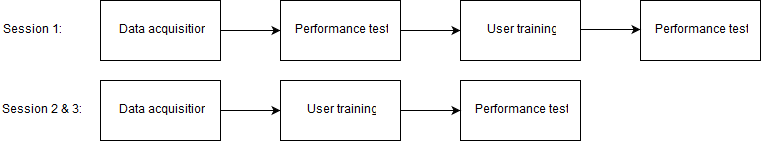
\includegraphics[width=0.9\textwidth]{figures/pMethods/experiment_protocol_pipeline}  
	\caption{Pipeline for the three sessions in the experiment and what steps each session contains.}
	\label{fig:experiment_protocol_pipeline} 
\end{figure}  


\textbf{Data acquisition}

For the myoelectric control system to be able to identify a performed movement as the movement that is actually performed, it needs information about how the movement looks when represented as a EMG signal. Thus, EMG data needs to be acquired from the forearm of the subject meanwhile the subject performs the movements that is used in the experiment, see \figref{fig:experiment_movements} on the last page. This data is fed to the control system for it to be able to recognize each movement. In this experiment EMG data will be acquired from the subject with an EMG-electrode armband: Myo armband(MYB) from Thalmic Labs. The chronology of this step is as follows:

\begin{enumerate}
	\item Apply MYB on dominant forearm at the thickest part.
	\item Synchronize MYB by performing wrist extension until three distinct vibrations are felt.
	\item Perform 15 seconds of maximum voluntary contraction (MVC) of instructed movement. Following the MVC the subject will be given a 15 seconds resting period to avoid muscle fatigue.
	\item Perform three 15 seconds contraction trails of respectively 40\%, 50\% and 60\% of MVC. During these contractions the subject will control a green marker representing the EMG signal and try to follow a trapezoidal trajectory as precise as possible. The trapezoidal trajectory consists of two five second transition phases and one five second plateau phase. Between each trial the subject will be given a 10 seconds resting period to avoid muscle fatigue.
	\item Repeat step 3-4 until training data from all four wrist movements has been recorded.
\end{enumerate}

An illustration of the interface used for data acquisition is shown in \figref{fig:dataacqGUI}

\begin{figure}[H]                 
	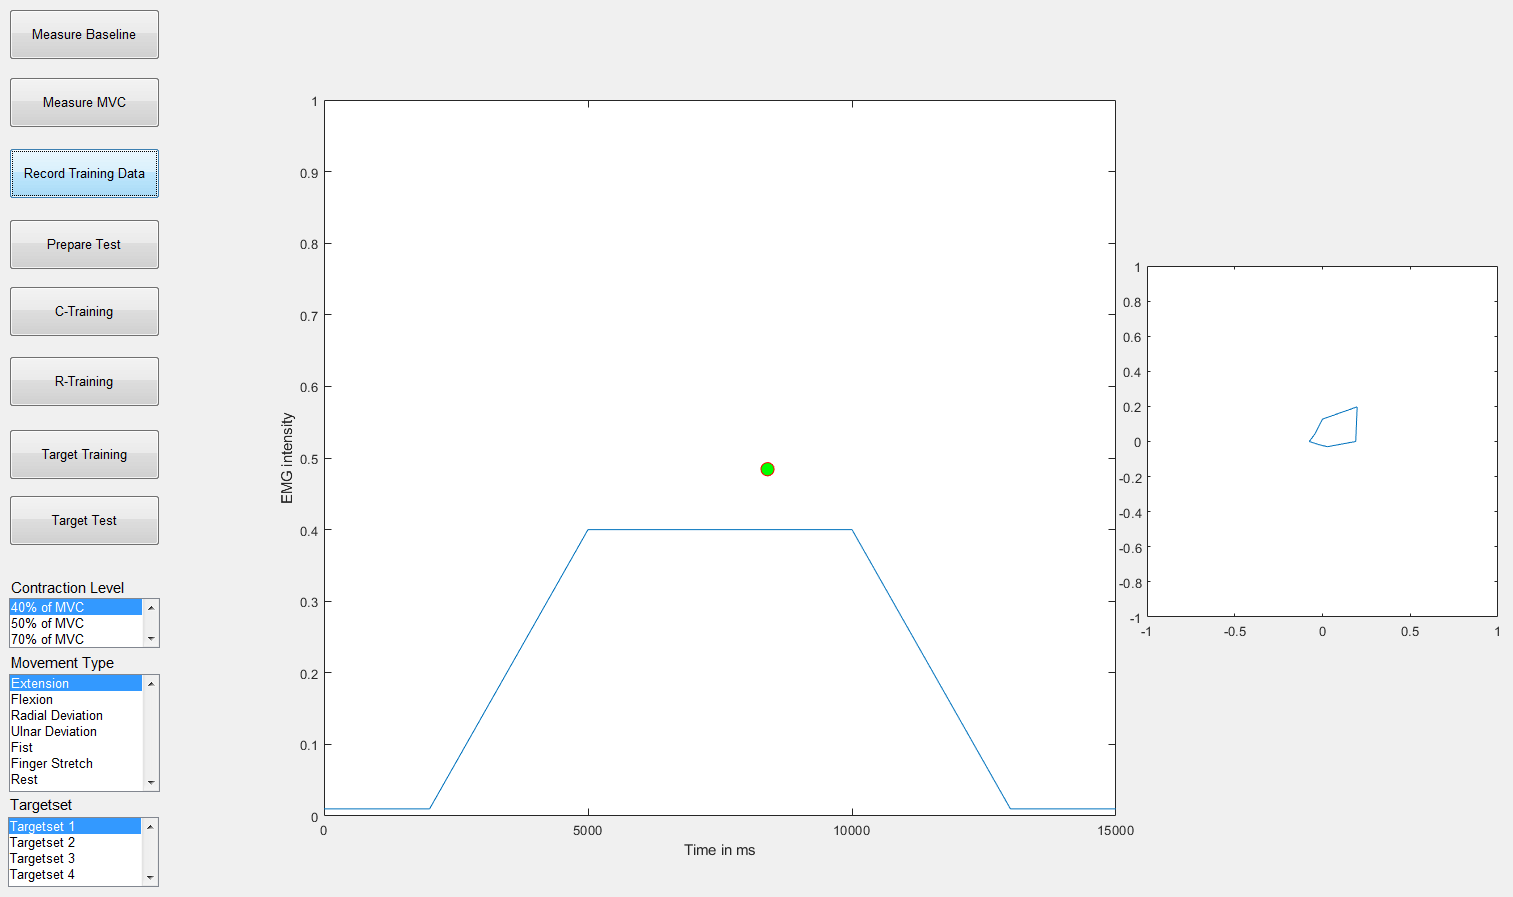
\includegraphics[width=.6\textwidth]{figures/xBackground/dataacqGUI}  
	\caption{Illustration of the data acquisition interface showing the trapezoidal trajectory and the green marker representing the EMG signal.}
	\label{fig:dataacqGUI} 
\end{figure}

\textbf{User training} %test group

The purpose of user training is for the subject to train the movements used in the performance test. During the user training the subject will train one movement at a time in different contraction levels. When training a movement, visual feedback in form of confidence levels on how well the control system recognizes movements, is shown in percentage in a bar plot. In addition, the level of contraction is shown in a text box above the bar plot. When performing the instructed movement at the instructed level of contraction the background colour of the text box will appear green; if it is within the instructed level it appears red. The aim for the subject is to reach and withhold the instructed contraction level with 100 \% recognition certainty for each movement. The chronology of this step is as follows:

\begin{enumerate}
	\item Perform flexion at 15-25 \% contraction level for 20 seconds followed by 10 seconds rest.
	\item Perform extension at 15-25 \% contraction level for 20 seconds followed by 10 seconds rest.
	\item Perform radial deviation at 15-25 \% contraction level for 20 seconds followed by 10 seconds rest.
	\item Perform ulnar deviation at 15-25 \% contraction level for 20 seconds followed by 10 seconds rest.
	\item Perform open hand movement at 15-25 \% contraction level for 20 seconds followed by 10 seconds rest.
	\item Perform closed hand movement at 15-25 \% contraction level for 20 seconds followed by 10 seconds rest.
	%\item Perform instructed movement smoothly increasing the contraction level from 30 \% to 70 \% within x seconds. When reaching the 70 \% contraction level the subject decreases the contraction level to 30 \% within x seconds.
	\item Repeat step 1-6 at 35-45 \% contraction level.
	\item Repeat step 1-6 at 55-65 \% contraction level.
	\item Repeat step 1-6 at 75-85 \% contraction level.
\end{enumerate} 

An illustration of the interface used for user training is shown in \figref{fig:usertraintestGUI}

\begin{figure}[H]                 
	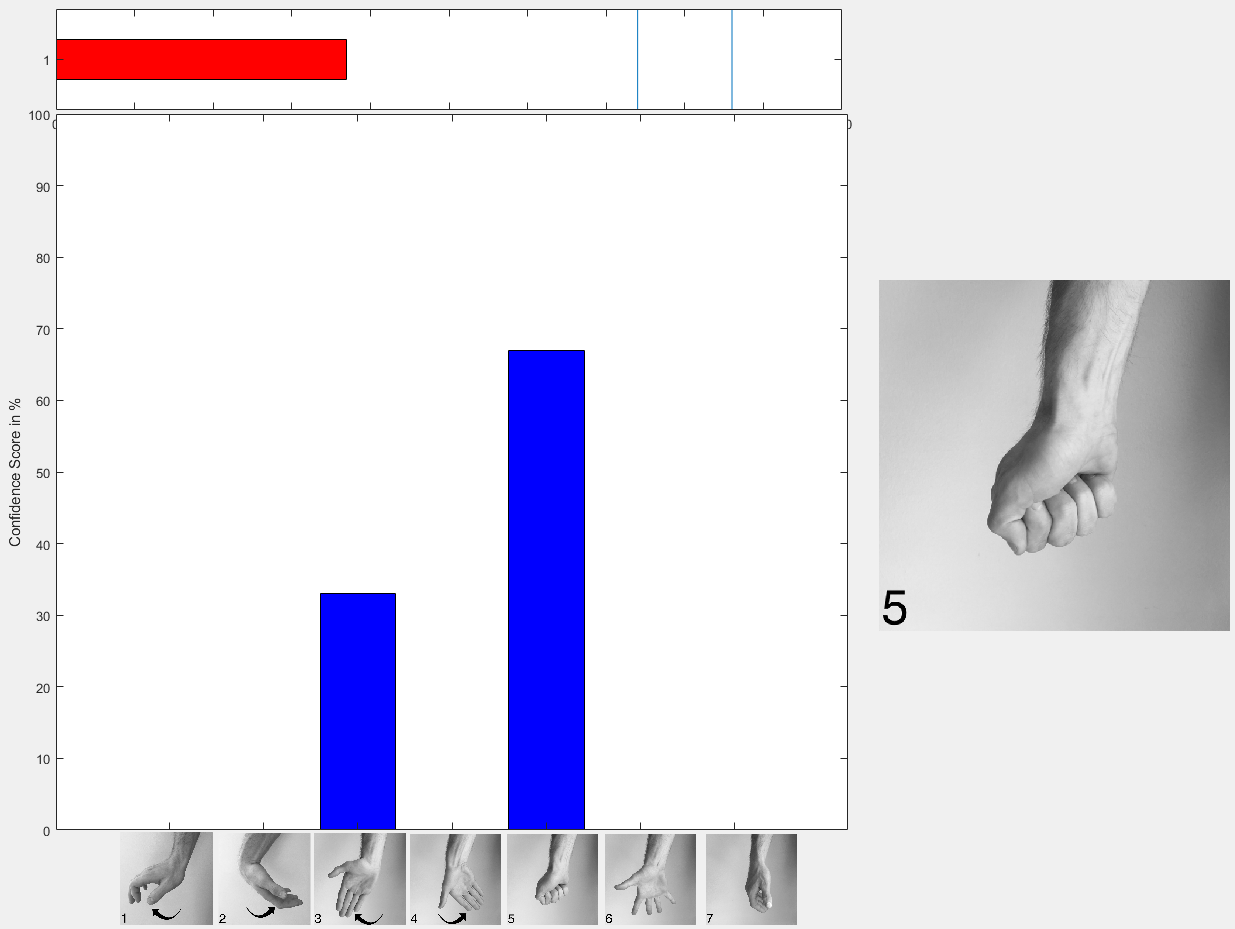
\includegraphics[width=.6\textwidth]{figures/xBackground/usertraintestGUI}  
	\caption{Illustration of the user training interface showing the bar plot indicating the confidence level of movement recognition and the text box indicating contraction level.}
	\label{fig:usertraintestGUI} 
\end{figure}

\textbf{User Training} %control group

The purpose of user training is for the subject to train the movements used in the performance test. During the user training the subject will train one movement at a time in different contraction levels. When training a movement, visual feedback on which movement the control system recognizes, is shown in percentage in a bar plot. In addition, the level of contraction is shown in a text box above the bar plot. When performing the instructed movement at the instructed level of contraction the background colour of the text box will appear green; if it is within the instructed level it appears red. The aim for the subject is to reach and withhold the instructed contraction level with 100 \% recognition certainty for each movement. The chronology of this step is as follows:

\begin{enumerate}
	\item Perform flexion at 15-25 \% contraction level for 20 seconds followed by 10 seconds rest.
	\item Perform extension at 15-25 \% contraction level for 20 seconds followed by 10 seconds rest.
	\item Perform radial deviation at 15-25 \% contraction level for 20 seconds followed by 10 seconds rest.
	\item Perform ulnar deviation at 15-25 \% contraction level for 20 seconds followed by 10 seconds rest.
	\item Perform open hand movement at 15-25 \% contraction level for 20 seconds followed by 10 seconds rest.
	\item Perform closed hand movement at 15-25 \% contraction level for 20 seconds followed by 10 seconds rest.
	%\item Perform instructed movement smoothly increasing the contraction level from 30 \% to 70 \% within x seconds. When reaching the 70 \% contraction level the subject decreases the contraction level to 30 \% within x seconds.
	\item Repeat step 1-6 at 35-45 \% contraction level.
	\item Repeat step 1-6 at 55-65 \% contraction level.
	\item Repeat step 1-6 at 75-85 \% contraction level.
\end{enumerate} 

An illustration of the interface used for user training is shown in \figref{fig:usertraincontrolGUI}

\begin{figure}[H]                 
	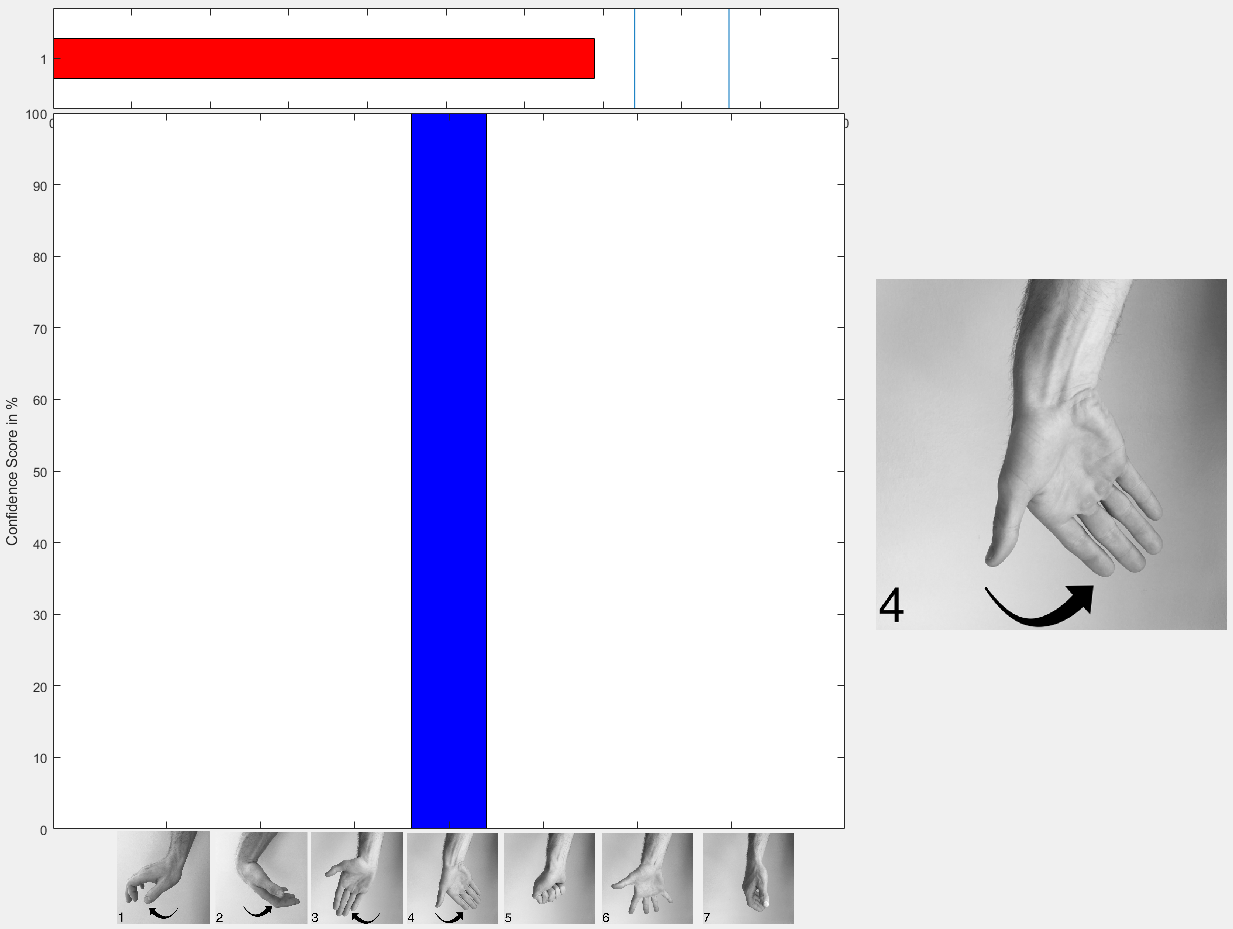
\includegraphics[width=.6\textwidth]{figures/xBackground/usertraincontrolGUI}  
	\caption{Illustration of the user training interface showing the bar plot indicating which movement is being recognized and the text box indicating contraction level.}
	\label{fig:usertraincontrolGUI} 
\end{figure}

\textbf{Performance test}

The purpose of the performance test is to assess the subject's ability to control a prosthesis. Instead of doing a test with a real prosthesis a virtual alternative has been developed for this experiment. The prosthesis is represented as a red circular cursor in a Cartesian coordinate system, which the subject can move as well as expand and shrink in size by performing the trained movement. The following bullets describe which movement corresponds to which action in the coordinate system:

\begin{itemize}
	\item Flexion moves the cursor left.
	\item Extension moves the cursor right.
	\item Radial deviation moves the cursor up.
	\item Ulnar deviation moves the cursor down.
	\item Open hand expands the cursor.
	\item Closed hand shrinks the cursor.
	\item Rest keeps the cursor still.
\end{itemize}

 The performance test consists of a target reaching test, where the subject must reach 16 targets of different sizes and locations. Only one target will be visible at a time. For the subject to reach a target and make a new appear, the subject must center the cursor in the center of the target and expand/shrink the cursor to fit the size of the target. The cursor will appear green, when located at the correct position. The subject must dwell the cursor in a target for 1 seconds for it to be reached. When the cursor has dwelled for 1 second, it will appear blue for 1 second to indicate that the target has been reached. If this is not done within 15 seconds a new target will appear. The aim for the subject is to reach as many target as possible as quickly as possible. The subject is only able to perform one movement at a time, as trained in the user training. Thus, no simultaneously performed movements will be recognized by the control system. The chronology of this step is as follows:

\begin{enumerate}
	\item Reach the visible target.
	\item Repeat step 1 until all targets have been shown.
\end{enumerate}

An illustration of the interface used for the performance test is shown in \figref{fig:perftestGUI}

\begin{figure}[H]                 
	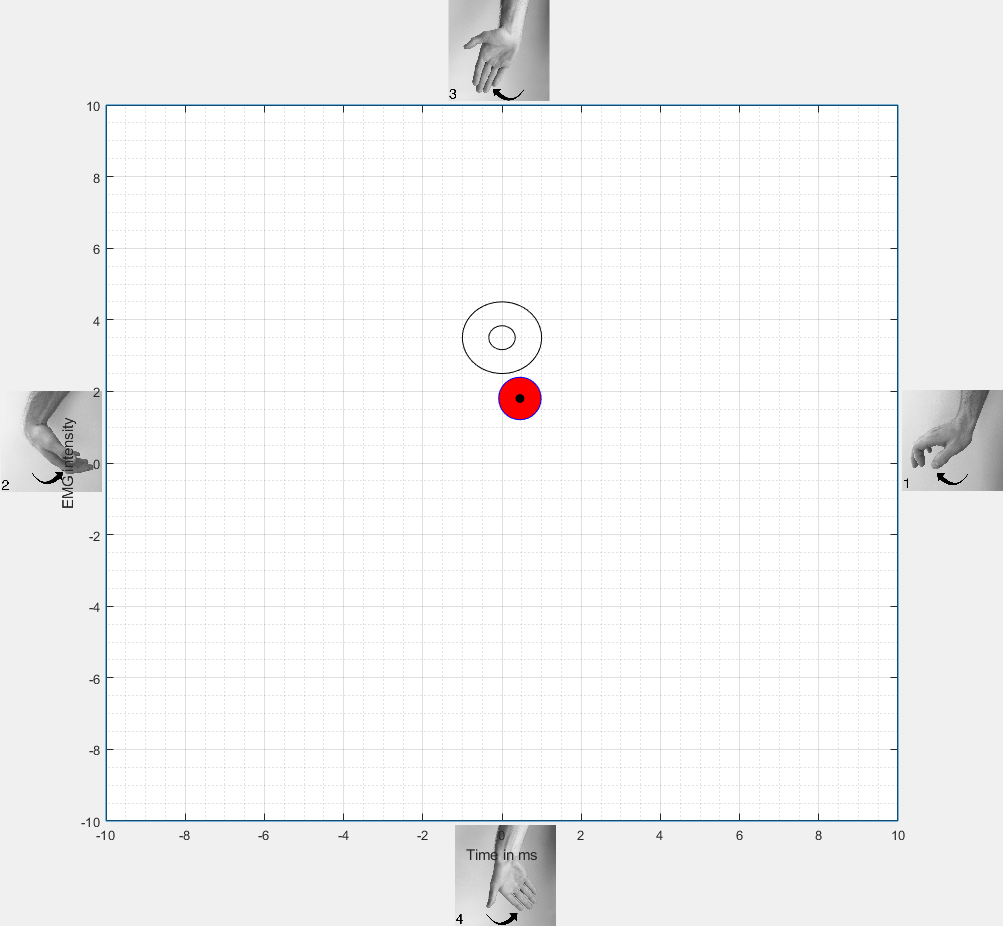
\includegraphics[width=.6\textwidth]{figures/xBackground/perftestGUI}  
	\caption{Illustration of the performance test interface showing a target and the cursor representing the prosthesis output.}
	\label{fig:perftestGUI} 
\end{figure}

\textbf{Movements used in the experiment}

\begin{figure}[H]                 
	\includegraphics[width=.6\textwidth]{figures/xBackground/fig:experiment_movements}  
	\caption{Illustration of the movements used in the experiment. 1: flexion, 2: extension, 3: radial deviation, 4: ulnar deviation, 5: open hand, 6: closed hand and 7: rest}
	\label{fig:experiment_movements} 
\end{figure}
%
%Session 1) Data acquisition, user training and performance test and 2) new training data acquisition and performance test. During the training data acquisition EMG data will be recorded from the subject with an EMG-electrode armband (Myo armband from Thalmic Labs) when performing four different wrist movements(flexion, extension, radial deviation and ulnar deviation) as illustrated in \figref{FIGURE}. The data is subsequently used to fit a classification model used in the myoelectric control scheme for the following user training and performance test. Before the performance test the user is given a training period to get familiar with wrist movements used in the performance test. During the performance test the subject will perform a target-reaching task in a cartesian coordinate system of reaching a number of targets using the trained movements by controlling a cursor representing the EMG. Each axis represent one of the four wrist movements, as seen in figure \figref{FIGURE2}, and the open/close hand movements expands/contracts the size of the cursor. The aim for the subject is to reach as many targets as quickly as possible. The subject will perform the target-reaching task twice - one in each session. The subjects are divided into two groups: a test group and a control group. As the study is single-blinded the subject will not be informed which group he/she belongs to.
%
%Chronology of session 1):
%\begin{enumerate}
%	\item Apply MYB on dominant forearm at the thickest part.
%	\item Synchronize MYB by performing wrist extension until three distinct vibrations are felt.
%	\item Perform 15 seconds of maximum voluntary contraction (MVC) of instructed movement. Following the MVC the subject will be given a 30 resting period to avoid fatigue.
%	\item Perform 15 seconds contractions of respectively 20\%, 40\% and 60\% of MVC. During these contractions the subject will control a green marker representing the EMG signal and try to follow a trapezoidal trajectory a precise as possible. The trapezoidal trajectory consists of two five second transition phases and one five second plateau phase as illustrated in figure \figref{FIGURE3}. Between each trial the subject will be given a 15 seconds resting period to avoid muscle fatigue.
%	\item Repeat step 3-4 until training data from all four wrist movements has been recorded.
%	\item The subject will train the seven movements. Each movement will be performed 10 times, where each single movement consists of a five second movement with increased intensity. To improve the precision of movements the subject will receive visual feedback consisting of the probability the movement to belong to based on the classifier. The ideal probability during the training is a 100\% probability of belonging to the trained movement and a 0\% probability of belonging to the remaining movements. 
%	\item The subject will perform a target-reaching task. The subject will control an cursor  in a cartesian coordinate system representing the features extracted from the EMG data, where the length represent the intensity and direction depicts the movement performed. To reach a target the subject must dwell the head of the arrow within the target for 0.5 seconds. If this is achieved the target will disappear. The target will similarly disappear if the subject fails to achieve this within 15 seconds. When an outer target disappears a target centred in origo appears and the subject must reach this before a new outer target appears. This procedure is continued until no more targets are shown. After finishing the performance test the subject will be given a 2 minutes resting period.
%\end{enumerate}
%
%
%Chronology of session 2):
%\begin{enumerate}
%	 \item Perform step 3-5 from session 1.
%	 \item Perform step 7 from session 1. 
%\end{enumerate}
% 







